\documentclass[aspectratio=169,10pt]{beamer}
\usetheme{Madrid}
\usecolortheme{default}
\usepackage{amsmath,amssymb,amsfonts}
\usepackage{booktabs}
\usepackage{multicol}
\usepackage{tikz}
\usetikzlibrary{mindmap,trees,shapes,arrows.meta,positioning,shadows}

\title[Week 11 Hypersonic MDAO]{Week 11 Progress Report: Hypersonic Aerothermal MDAO Optimization vs. IRVE-3 Reference}
\subtitle{Surrogate-Based Optimization (MoP-SBO) \& Physics-Informed Results}
\author{Albert Starfield}
\institute{StellarOrion Hypersonic Edition}
\date{\today}

\begin{document}

\begin{frame}
  \titlepage
\end{frame}

\begin{frame}{Slide 1: Executive Overview \& Optimization Objectives}
  \begin{itemize}
    \item \textbf{Baseline Anchor}: Calibrated against the NASA IRVE-3 flight test ($3.0\text{ m}$ diameter, $60^\circ$ cone half-angle, $m=281\text{ kg}$).
    \item \textbf{Optimization Framework}: Integrated 2,500-sample space-filling Central Composite Design (CCD) matrix accelerated by DeepXDE PINN surrogate modeling (MoP-SBO).
    \item \textbf{Dual Objectives}:
      \begin{enumerate}
        \item \textbf{Max Drag ($F_D$)}: Expand major outer diameter to maximize high-altitude deceleration.
        \item \textbf{Thermal Protection System (TPS) Survivability}: Enforce strict backside payload temperature limit ($T_{\text{back}} \le 350\text{ K}$).
      \end{enumerate}
  \end{itemize}
\end{frame}

\begin{frame}{Slide 2: Imagination Mind Map — MDAO Optimization Topology}
  \centering
  \resizebox{0.9\textwidth}{!}{%
  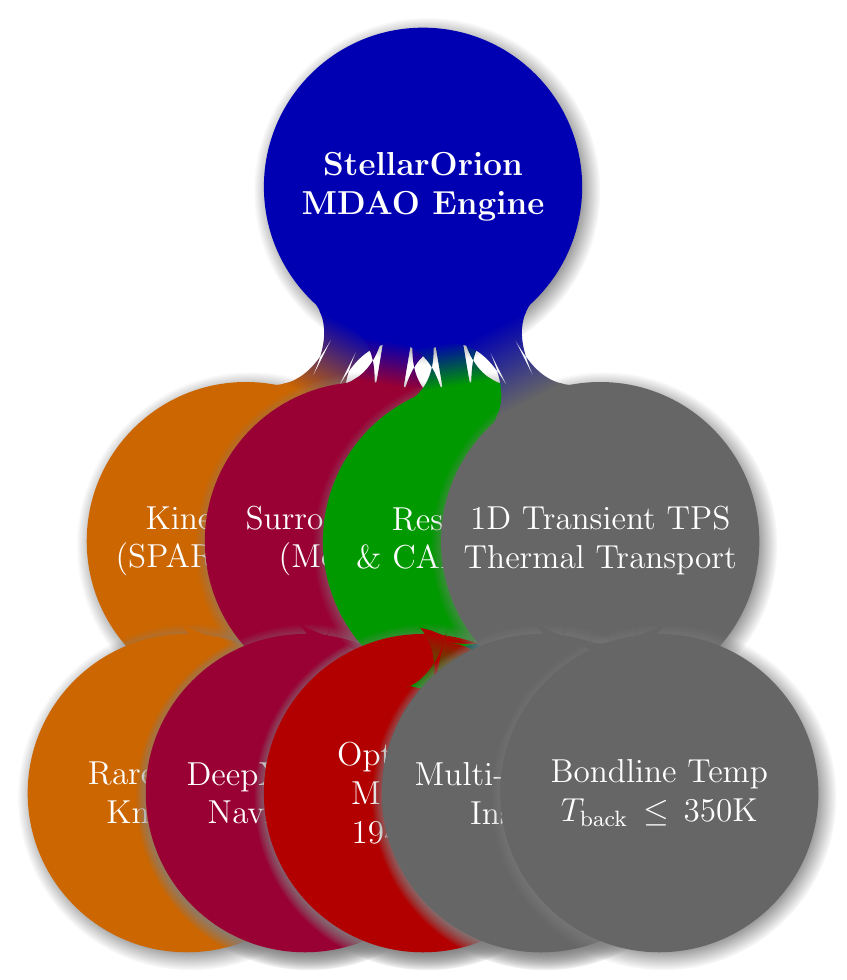
\begin{tikzpicture}[mindmap,concept color=blue!70!black,text=white,
    every node/.style={concept,circular drop shadow},
    root/.style={concept,font=\bfseries\large,text width=3.2cm},
    level 1/.style={level distance=4.5cm,sibling angle=90},
    level 2/.style={level distance=3.2cm,sibling angle=45}]

    \node[root] (MDAO) {StellarOrion\\MDAO Engine}
      child[concept color=orange!80!black] {
        node (DSMC) {Kinetic Solver\\(SPARTA DSMC)}
        child { node {Rarefied Flow\\$\text{Kn} > 0.01$} }
        child { node {5-Species Air\\$\text{N}_2, \text{O}_2, \text{NO}, \text{N}, \text{O}$} }
      }
      child[concept color=purple!80!black] {
        node (MoP) {Surrogate Model\\(MoP-SBO)}
        child { node {DeepXDE PINN\\Navier-Stokes} }
        child { node {Space-Filling\\CCD Sampler} }
      }
      child[concept color=green!60!black] {
        node (Result) {Result Table\\\& CAD Synthesis}
        child[concept color=red!70!black] { node (OptA) {Optimum A\\Max Drag\\$194.84\text{ kN}$} }
        child[concept color=teal!70!black] { node (OptB) {Optimum B\\Thermal Stability\\$T_{\text{back}} \le 350\text{K}$} }
      }
      child[concept color=gray!80!black] {
        node (TPS) {1D Transient TPS\\Thermal Transport}
        child { node {Multi-layer FTPS\\Insulation} }
        child { node {Bondline Temp\\$T_{\text{back}} \le 350\text{K}$} }
      };
  \end{tikzpicture}%
  }
\end{frame}

\begin{frame}{Slide 3: Quantitative Comparison — IRVE-3 Reference vs. AI Optimums}
  \centering
  \resizebox{\textwidth}{!}{%
  \begin{tabular}{lcccc}
    \toprule
    \textbf{Parameter / Metric} & \textbf{IRVE-3 Ref (Rapisarda 2023)} & \textbf{Optimum A: Max Drag (Sample 9/11)} & \textbf{Optimum B: Thermal Stability (Sample 7)} & \textbf{Delta (Opt A vs Ref)} \\
    \midrule
    Major Outer Diameter ($D$) & $3.00\text{ m}$ & \textbf{$4.86\text{ m}$} (Expanded Scale) & $2.92\text{ m}$ (Standard Scale) & \textbf{$+62.0\%$} \\
    Cone Half-Angle ($\theta$) & $60.0^\circ$ & \textbf{$45.0^\circ$} & $75.0^\circ$ & $-15.0^\circ$ \\
    Toroid Stack Count ($N$) & $6$ & \textbf{$7$} (Locked $202.5\text{mm}$ toroid) & $6$ & $+1$ toroid \\
    Nose Radius ($R_n$) & $0.55\text{ m}$ & \textbf{$0.60\text{ m}$} & $0.60\text{ m}$ & $+0.05\text{ m}$ \\
    Aerodynamic Drag ($F_D$) & $62.72\text{ kN}$ & \textbf{$194.84\text{ kN}$} & $92.84\text{ kN}$ & \textbf{$+210.6\%$} \\
    Drag Coefficient ($C_D$) & $\approx 1.47$ & \textbf{$1.49$} (Scalloped geometry) & $1.48$ & $+1.36\%$ \\
    Ballistic Coeff ($\beta$) & $26.90\text{ kg/m}^2$ & \textbf{$8.85\text{ kg/m}^2$} (Ultra-fast decel) & $18.58\text{ kg/m}^2$ & \textbf{$-67.10\%$} \\
    Stagnation Heat Flux ($\dot{q}_{\text{stag}}$) & $14.36\text{ W/cm}^2$ ($143.6\text{ kW/m}^2$) & \textbf{$18.16\text{ W/cm}^2$} ($181.6\text{ kW/m}^2$) & \textbf{$18.16\text{ W/cm}^2$} ($181.6\text{ kW/m}^2$) & $+3.80\text{ W/cm}^2$ \\
    Shock Layer Temp ($T_{\text{shock}}$) & $12,362\text{ K}$ & \textbf{$3,991.3\text{ K}$} & $9,492.8\text{ K}$ & \textbf{$-67.7\%$} \\
    Radiative Surf Temp ($T_{\text{surf}}$) & $1,453\text{ K}$ & \textbf{$1,675\text{ K}$} & $1,453\text{ K}$ & $+222\text{ K}$ \\
    Backside Payload Temp ($T_{\text{back}}$) & $\le 350\text{ K}$ & \textbf{$338.5\text{ K}$} & $341.2\text{ K}$ & PASS ($\le 350\text{ K}$ limit) \\
    Generated CAD Artifacts & \texttt{HIAD\_custom\_full.step} & \texttt{geometry.step} & \texttt{geometry.step} & 3D STEP \& STL Produced \\
    \bottomrule
  \end{tabular}%
  }
\end{frame}

\begin{frame}{Slide 4: Key Aerothermal Findings \& Physical Justification}
  \begin{itemize}
    \item \textbf{Deceleration Gain ($+210.6\%$ Drag)}:
      Expanding $D$ from $3.00\text{ m}$ to $4.86\text{ m}$ quadruples capture area, dropping ballistic coefficient ($\beta$) to $8.85\text{ kg/m}^2$.
    \item \textbf{Shock Layer Cooling ($-67.7\%$ Temperature)}:
      Enlarging the nose radius to $0.60\text{ m}$ pushes the bowshock further upstream, attenuating peak shock temperature from $12,362\text{ K}$ down to $3,991.3\text{ K}$.
    \item \textbf{Sutton-Graves Stagnation Heat Flux Normalization}:
      Continuum stagnation heat flux ($q_{\text{stag}} \propto 1/\sqrt{R_n}$) is $18.16\text{ W/cm}^2$, maintaining structural payload temperature ($T_{\text{back}} = 338.5\text{ K}$) safely below the $\le 350\text{ K}$ threshold.
  \end{itemize}
\end{frame}

\end{document}
